\subsubsection{Signal conditioner (Galileo E1 + E5a)}


\begin{table}[H]
  \centering
  \footnotesize
  \resizebox{\ifdim\width>\linewidth\linewidth\else\width\fi}{!}{%
  \begin{tabular}{l>{\centering\arraybackslash}p{4.2cm}>{\centering\arraybackslash}p{4.2cm}}
    \hline
    \textbf{Channel} & \textbf{ch0 (Galileo E1)} & \textbf{ch1 (Galileo E5a)} \\
    \hline
    File format & ci8 & ci8 \\
    Source item type & ibyte & ibyte \\
    Data type adapter & Ibyte\_To\_Complex & Ibyte\_To\_Complex \\
    Input filter & Pass\_Through & Pass\_Through \\
    Resampling & $\times$5 zero-order hold, offline (\texttt{upsample\_iq.py}) & Pass\_Through \\
    Rate [MS/s] & 4 $\to$ 20 & 20 $\to$ 20 \\
    \hline
  \end{tabular}}
  \caption{Signal conditioner: recorded format and rate to gnss-sdr's internal \texttt{gr\_complex} stream; both bands are read in lockstep by one \texttt{Multichannel\_File\_Signal\_Source}.}
\end{table}

\subsubsection{Acquisition (Galileo E1 + E5a)}
Two-dimensional search over code delay and Doppler (one channel per band dumped; the others behave alike).

\begin{figure}[H]
  \centering
  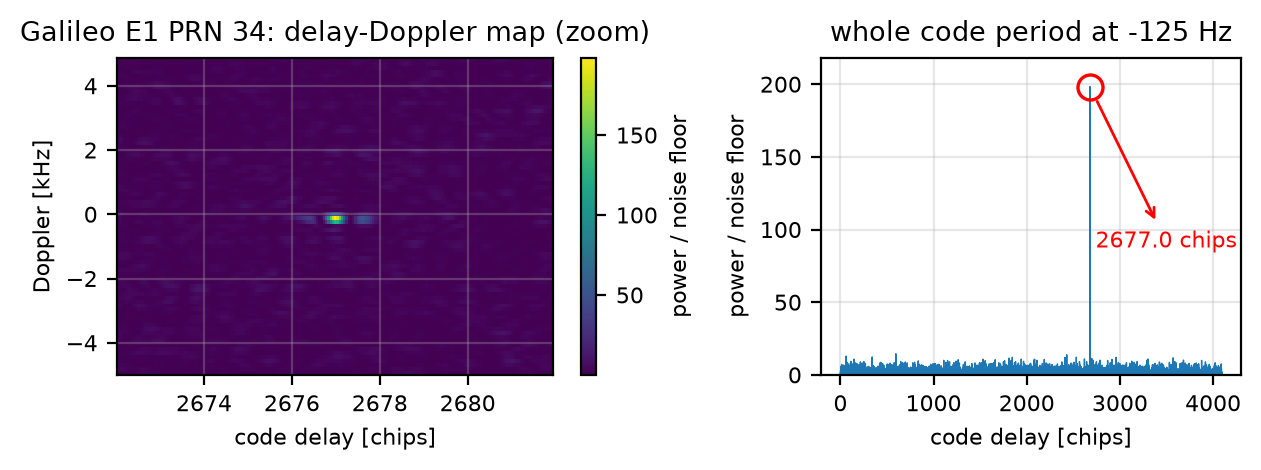
\includegraphics[width=1.0\linewidth]{gnss_sdr/x310_20261022T190000Z/galileo_acq_1B.png}
  \caption{Acquisition, Galileo E1: delay--Doppler search of PRN 34; one sharp peak (test statistic 272 vs threshold 52) at -125~Hz and 2677.0~chips.}
\end{figure}

\begin{figure}[H]
  \centering
  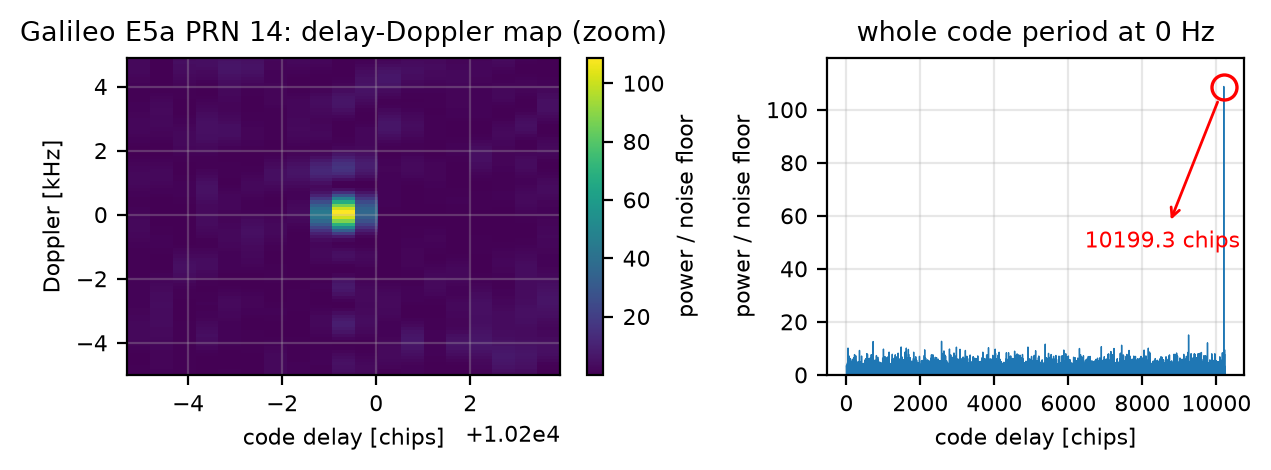
\includegraphics[width=1.0\linewidth]{gnss_sdr/x310_20261022T190000Z/galileo_acq_5X.png}
  \caption{Acquisition, Galileo E5a: delay--Doppler search of PRN 14; one sharp peak (test statistic 149 vs threshold 49) at -1427~Hz and 10199.3~chips.}
\end{figure}

\begin{table}[H]
  \centering
  \footnotesize
  \resizebox{\ifdim\width>\linewidth\linewidth\else\width\fi}{!}{%
  \begin{tabular}{lrrrr}
    \hline
    \textbf{Band} & \textbf{Attempts} & \textbf{Detections} & \textbf{Detected PRNs} & \textbf{Best statistic / threshold} \\
    \hline
    Galileo E1 & 5 & 1 & 34 & 5.3 \\
    Galileo E5a & 2 & 2 & 14 & 3.0 \\
    \hline
  \end{tabular}}
  \caption{Acquisition: search attempts of the dumped channel. Attempts on satellites that are not in view (or do not broadcast that signal, e.g. older GPS satellites on L5/L2C) are rejected below the threshold.}
\end{table}

\subsubsection{Tracking (Galileo E1 + E5a)}


\begin{figure}[H]
  \centering
  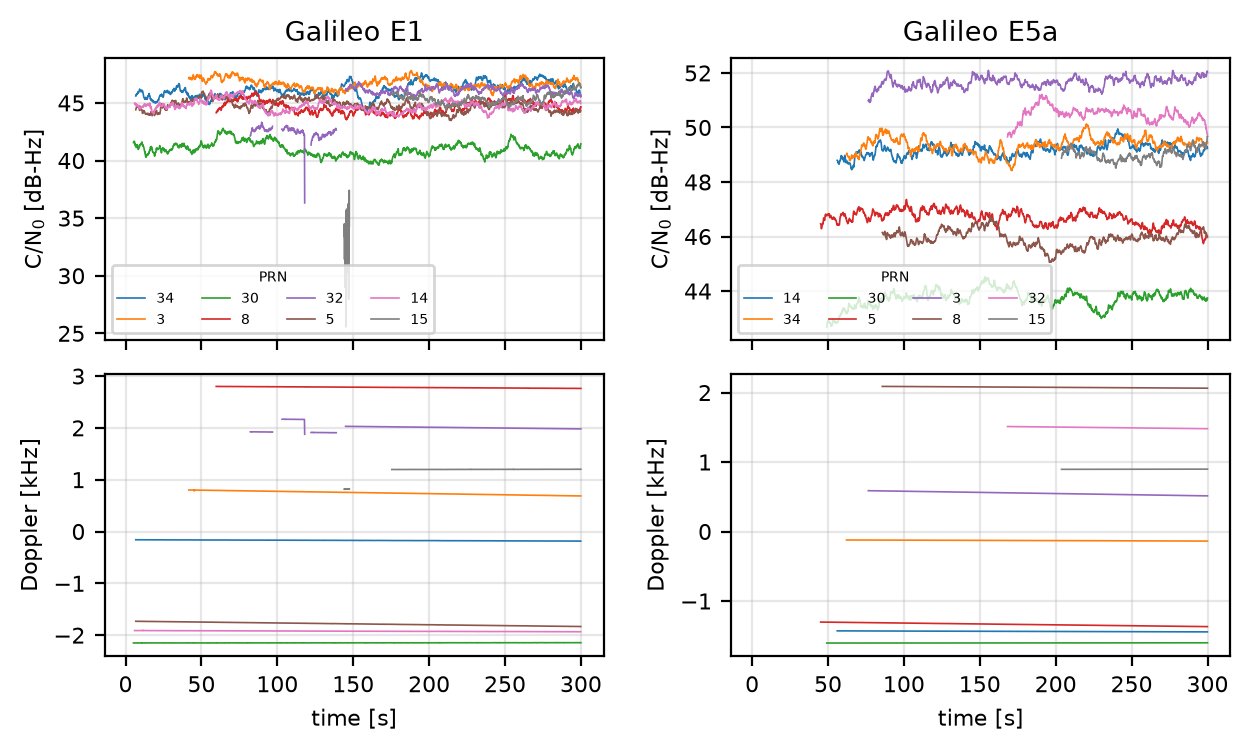
\includegraphics[width=1.0\linewidth]{gnss_sdr/x310_20261022T190000Z/galileo_tracking.png}
  \caption{Tracking: carrier-to-noise density ratio and carrier Doppler per satellite, while phase-locked (smooth Doppler curves = loops following the real satellite motion).}
\end{figure}

\begin{figure}[H]
  \centering
  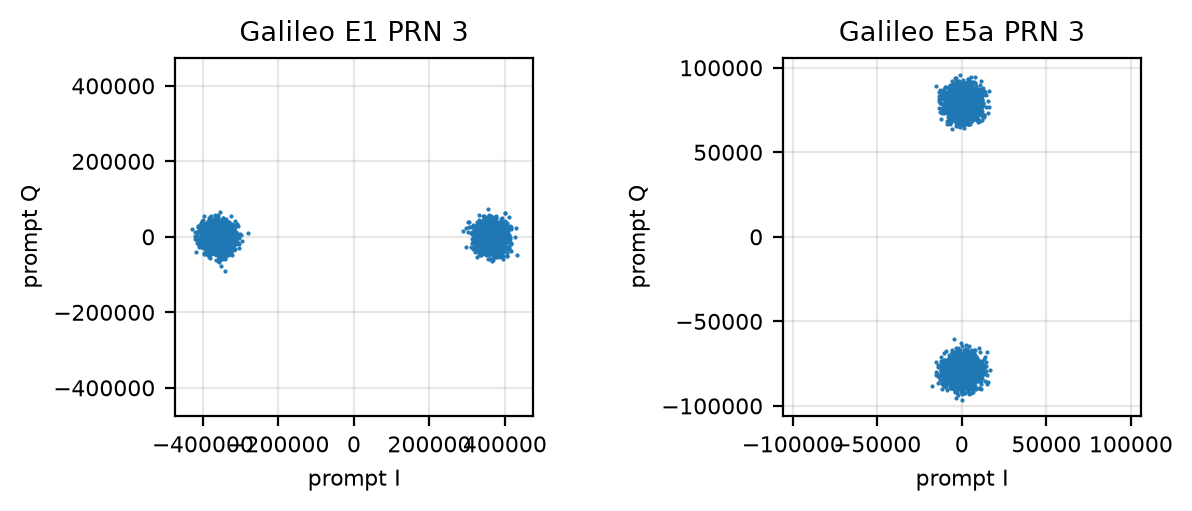
\includegraphics[width=1.0\linewidth]{gnss_sdr/x310_20261022T190000Z/galileo_tracking_iq.png}
  \caption{Tracking: prompt correlator outputs of the strongest satellite per band. Two tight clusters on one axis (the $\pm1$ data bits; GNSS-SDR's L5 tracking puts the data component on the Q axis), or a single one for a dataless pilot (Galileo E1-C and E5a-Q, tracked here), mean the PLL is phase-locked; a ring would mean it is not. \texttt{Prompt\_I}/\texttt{Prompt\_Q} are 32-bit floats (sums of the samples over one integration period, in file units): they never clip, only overflowing beyond $\pm 3.4\times10^{38}$, far above the $N\cdot\text{full scale}\cdot\sqrt{2}$ a sum of $N$ samples can reach.}
\end{figure}

\begin{table}[H]
  \centering
  \footnotesize
  \resizebox{\ifdim\width>\linewidth\linewidth\else\width\fi}{!}{%
  \begin{tabular}{lrrrrrr}
    \hline
    \textbf{Band} & \textbf{Ch.} & \textbf{PRN} & \textbf{Median C/N$_0$ [dB-Hz]} & \textbf{Phase-locked [\%]} & \textbf{Losses of lock} & \textbf{Tracked [s]} \\
    \hline
    Galileo E1 & 0 & 34 & 46.1 & 98 & 0 & 299 \\
    Galileo E1 & 1 & 3 & 46.6 & 87 & 2 & 298 \\
    Galileo E1 & 2 & 30 & 40.9 & 99 & 0 & 299 \\
    Galileo E1 & 3 & 8 & 44.4 & 81 & 2 & 298 \\
    Galileo E1 & 4 & 32 & 45.7 & 68 & 7 & 299 \\
    Galileo E1 & 5 & 5 & 44.8 & 98 & 0 & 298 \\
    Galileo E1 & 6 & 14 & 44.7 & 98 & 0 & 300 \\
    Galileo E1 & 7 & 15 & 44.5 & 43 & 8 & 300 \\
    Galileo E5a & 8 & 14 & 48.9 & 31 & 1 & 275 \\
    Galileo E5a & 9 & 34 & 48.9 & 30 & 1 & 274 \\
    Galileo E5a & 10 & 30 & 43.5 & 52 & 0 & 272 \\
    Galileo E5a & 11 & 5 & 46.8 & 53 & 0 & 274 \\
    Galileo E5a & 12 & 3 & 51.6 & 49 & 0 & 244 \\
    Galileo E5a & 13 & 8 & 45.9 & 48 & 0 & 235 \\
    Galileo E5a & 14 & 32 & 50.4 & 37 & 0 & 144 \\
    Galileo E5a & 15 & 15 & 49.0 & 30 & 0 & 114 \\
    \hline
  \end{tabular}}
  \caption{Tracking: per channel and satellite (phase-locked: carrier lock test $> 0.8$).}
\end{table}

\subsubsection{Telemetry decoder (Galileo E1 + E5a)}


\begin{figure}[H]
  \centering
  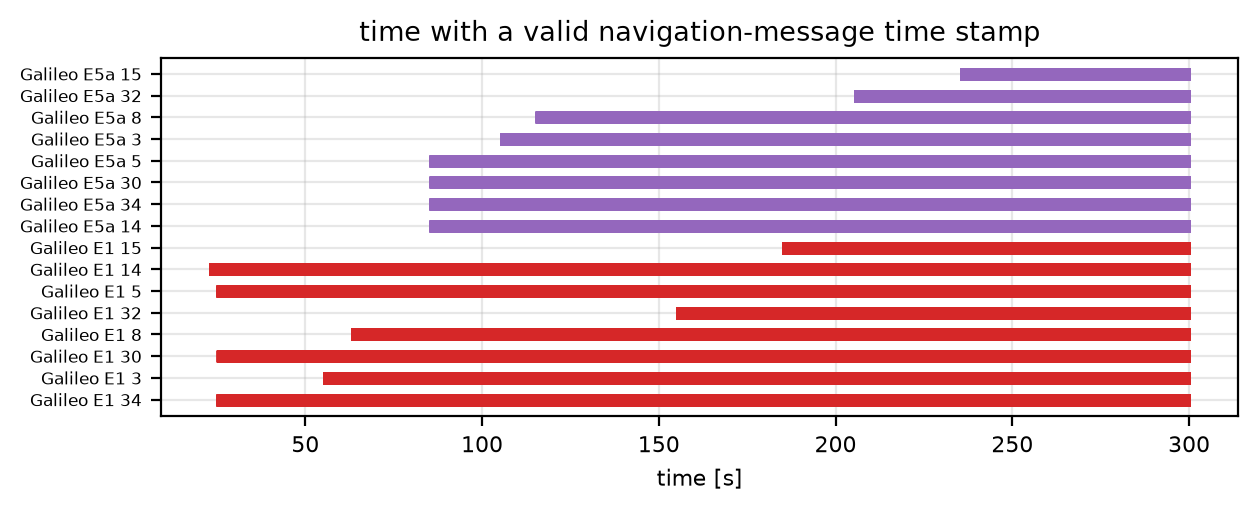
\includegraphics[width=1.0\linewidth]{gnss_sdr/x310_20261022T190000Z/galileo_telemetry.png}
  \caption{Telemetry decoder: per band and satellite, when the decoder delivered a valid transmit time (the first one comes after the first complete frame/message).}
\end{figure}

\begin{table}[H]
  \centering
  \footnotesize
  \resizebox{\ifdim\width>\linewidth\linewidth\else\width\fi}{!}{%
  \begin{tabular}{lrrrrr}
    \hline
    \textbf{Band} & \textbf{PRN} & \textbf{Messages decoded} & \textbf{Ephemeris} & \textbf{First valid at [s]} & \textbf{TOW [s]} \\
    \hline
    Galileo E1 & 3 & 24 & yes & 55.2 & 414080.0 \\
    Galileo E1 & 5 & 26 & yes & 25.2 & 414050.0 \\
    Galileo E1 & 8 & 23 & yes & 63.2 & 414088.0 \\
    Galileo E1 & 14 & 26 & yes & 23.2 & 414048.0 \\
    Galileo E1 & 15 & 10 & yes & 185.2 & 414210.0 \\
    Galileo E1 & 30 & 26 & yes & 25.2 & 414050.0 \\
    Galileo E1 & 32 & 13 & yes & 155.2 & 414180.0 \\
    Galileo E1 & 34 & 26 & yes & 25.2 & 414050.0 \\
    Galileo E5a & 3 & 11 & yes & 105.4 & 414130.3 \\
    Galileo E5a & 5 & 12 & yes & 85.4 & 414110.3 \\
    Galileo E5a & 8 & 10 & yes & 115.4 & 414140.3 \\
    Galileo E5a & 14 & 11 & yes & 85.4 & 414110.3 \\
    Galileo E5a & 15 & 3 & yes & 235.4 & 414260.3 \\
    Galileo E5a & 30 & 12 & yes & 85.4 & 414110.3 \\
    Galileo E5a & 32 & 5 & yes & 205.4 & 414230.3 \\
    Galileo E5a & 34 & 12 & yes & 85.4 & 414110.3 \\
    \hline
  \end{tabular}}
  \caption{Telemetry decoder: Galileo E1 I/NAV words, Galileo E5a F/NAV pages decoded, ephemeris obtained, and the first valid time of week.}
\end{table}

\subsubsection{Observables (Galileo E1 + E5a)}
Pseudorange, carrier phase and Doppler of every channel at common receiver epochs.

\begin{figure}[H]
  \centering
  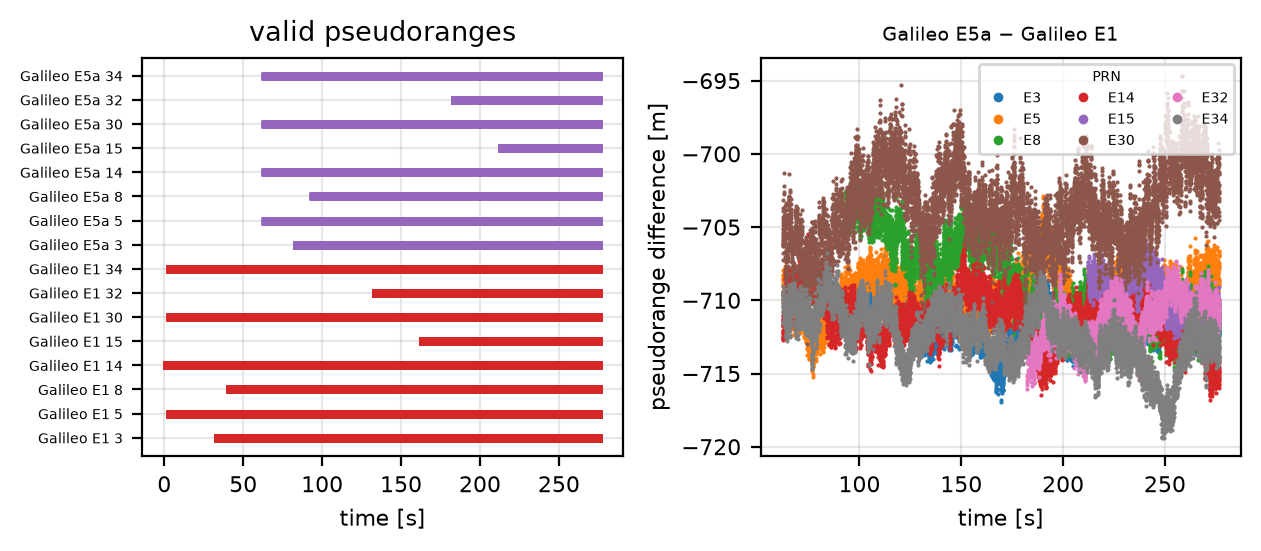
\includegraphics[width=1.0\linewidth]{gnss_sdr/x310_20261022T190000Z/galileo_observables.png}
  \caption{Observables: epochs with a valid pseudorange per band and satellite, and the difference between the two bands' pseudoranges of the same satellite (a constant receiver inter-band bias, the same for every satellite, plus the slowly varying ionospheric delay).}
\end{figure}

\begin{table}[H]
  \centering
  \footnotesize
  \resizebox{\ifdim\width>\linewidth\linewidth\else\width\fi}{!}{%
  \begin{tabular}{lrrrrrr}
    \hline
    \textbf{Difference} & \textbf{PRN} & \textbf{Common epochs} & \textbf{of run [\%]} & \textbf{Mean [m]} & \textbf{Std [m]} & \textbf{Drift [m/s]} \\
    \hline
    Galileo E5a $-$ Galileo E1 & 3 & 9563 & 64 & -711.43 & 1.45 & -0.0075 \\
    Galileo E5a $-$ Galileo E1 & 5 & 10437 & 70 & -709.61 & 1.55 & 0.0065 \\
    Galileo E5a $-$ Galileo E1 & 8 & 9128 & 61 & -708.81 & 2.89 & -0.0451 \\
    Galileo E5a $-$ Galileo E1 & 14 & 10437 & 70 & -711.16 & 1.64 & -0.0082 \\
    Galileo E5a $-$ Galileo E1 & 15 & 3147 & 21 & -709.62 & 1.46 & -0.0504 \\
    Galileo E5a $-$ Galileo E1 & 30 & 10457 & 70 & -703.72 & 2.59 & 0.0079 \\
    Galileo E5a $-$ Galileo E1 & 32 & 4647 & 31 & -711.39 & 1.51 & 0.0347 \\
    Galileo E5a $-$ Galileo E1 & 34 & 10437 & 70 & -712.45 & 1.88 & -0.0177 \\
    \hline
  \end{tabular}}
  \caption{Observables: pseudorange difference between the two bands of each satellite at common epochs (similar means = shared receiver bias; std = code noise of both bands).}
\end{table}

\subsubsection{PVT (Galileo E1 + E5a)}
Position from the pseudoranges and the decoded ephemeris, compared with the surveyed antenna position (-23.209433$^\circ$, -45.874875$^\circ$, 596.42~m).

\begin{figure}[H]
  \centering
  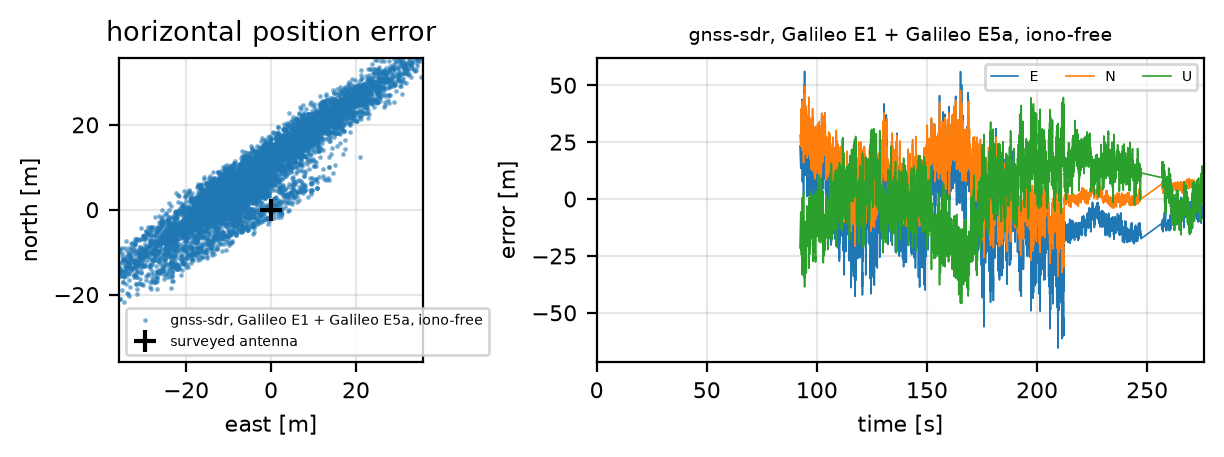
\includegraphics[width=1.0\linewidth]{gnss_sdr/x310_20261022T190000Z/galileo_pvt.png}
  \caption{PVT: position error with respect to the surveyed antenna position. gnss-sdr: GNSS-SDR's own RTKLIB solution.}
\end{figure}

\begin{table}[H]
  \centering
  \footnotesize
  \resizebox{\ifdim\width>\linewidth\linewidth\else\width\fi}{!}{%
  \begin{tabular}{l>{\centering\arraybackslash}p{4.2cm}}
    \hline
    \textbf{Solution} & \textbf{gnss-sdr, Galileo E1 + Galileo E5a, iono-free} \\
    \hline
    Solutions & 8642 \\
    Run with fix [\%] & 64 \\
    Mean E / N / U [m] & -4.8 / 6.7 / 2.8 \\
    Std E / N / U [m] & 15.5 / 11.9 / 14.2 \\
    RMS 2-D [m] & 21.2 \\
    RMS 3-D [m] & 25.6 \\
    95\% horiz. [m] & 40.3 \\
    \hline
  \end{tabular}}
  \caption{PVT: position error statistics with respect to the surveyed antenna (mean = accuracy, std = precision; \% of the run's seconds with a position; gnss-sdr outputs several solutions per second, gnss\_spp.py computes one per second).}
\end{table}

